\clearpage
\section{Experimentación Y Resultados}

\subsection{Introducción}
 Realizamos los experimentos en tres computadoras con procesadores similares y se trató de mantener cualquier otro programa cerrado. Igualmente cada conjunto de test fue resuelto en la misma máquina para que las diferencias sean lo más dependendientes a los inputs y los procesos posible.

\subsection{Caso básico}
A continuación plantearemos distintos casos de parabrisas con distintas granularidades que utlizaremos durante las pruebas. 

\begin{figure}[htb]

\minipage{0.5\textwidth}
\begin{center}
       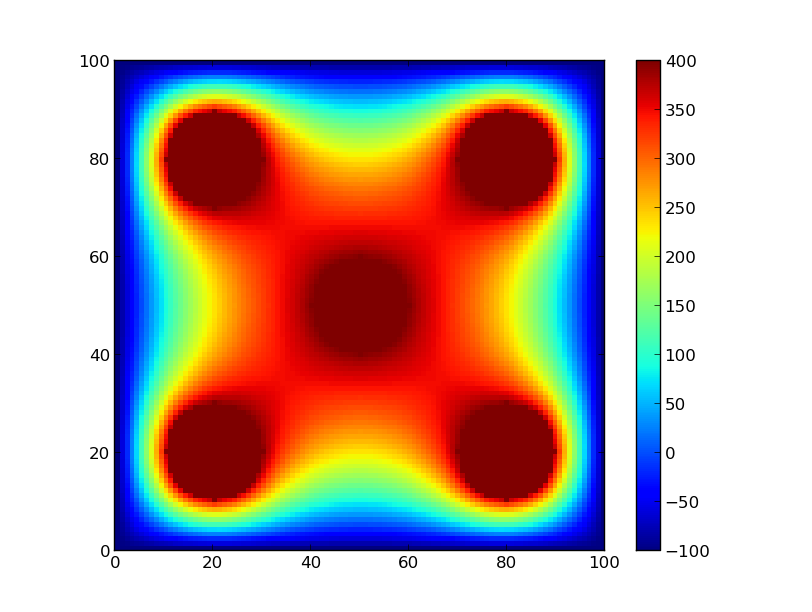
\includegraphics[scale=0.3]{imagenes/test5_gran1.png}
                \caption{Granularidad 1}
        \end{center}
\endminipage\hfill
\minipage{0.5\textwidth}
\begin{center}
        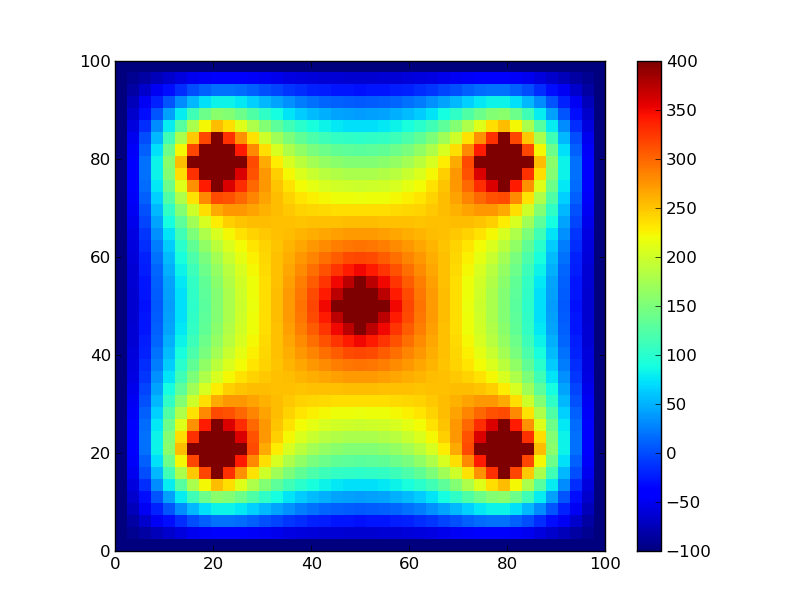
\includegraphics[scale=0.3]{imagenes/test5.png}
                \caption{Granularidad 2.5}
        \end{center}
\endminipage\hfill 
\end{figure}

\begin{figure}[!htb]
\minipage{0.5\textwidth}
\begin{center}
    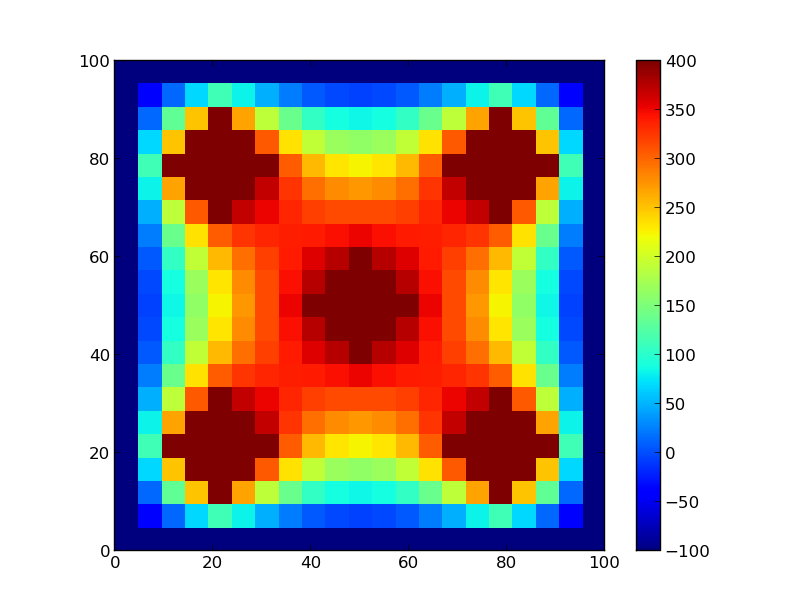
\includegraphics[scale=0.3]{imagenes/test5_gran5.png}
                \caption{Granularidad 5}
 \end{center}
\endminipage
\minipage{0.5\textwidth}
\begin{center}
   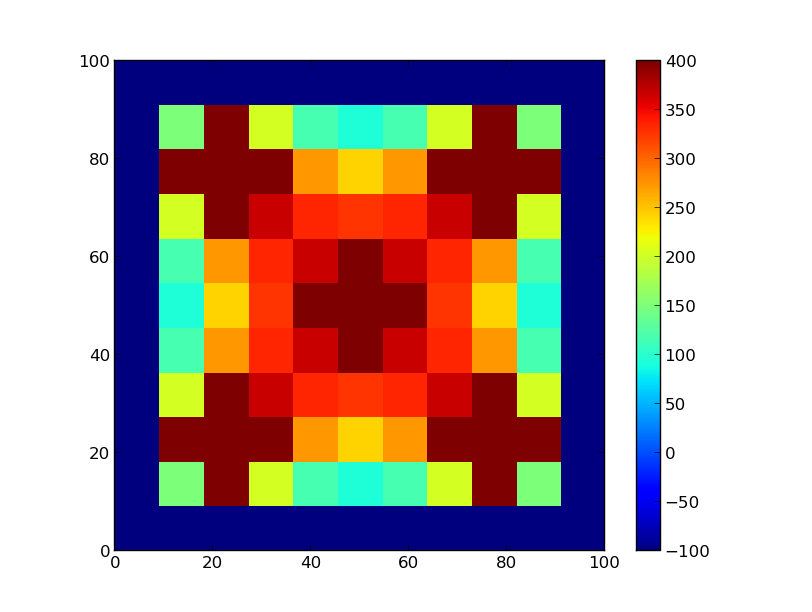
\includegraphics[scale=0.3]{imagenes/test5_gran10.png}
                \caption{Granularidad 10}
        \end{center}
\endminipage\hfill
\end{figure}
\clearpage

\subsubsection{Resultados Random}

A continuación observaremos un caso en la que la única sanguijuela que se debe eliminar es la del centro. Esta se encuentra exactamente en el punto central. Adicionalmente hay otras 4 sanguijuelas en las puntas. 
Matar a estas no soluciona nada ya que la del centro esta aplicando una temperatura constante de 400 Cº. Lo observaremos con 4 discretizaciones distintas para tener un mas amplio panorama.
\begin{figure}[htb]
\begin{center}
        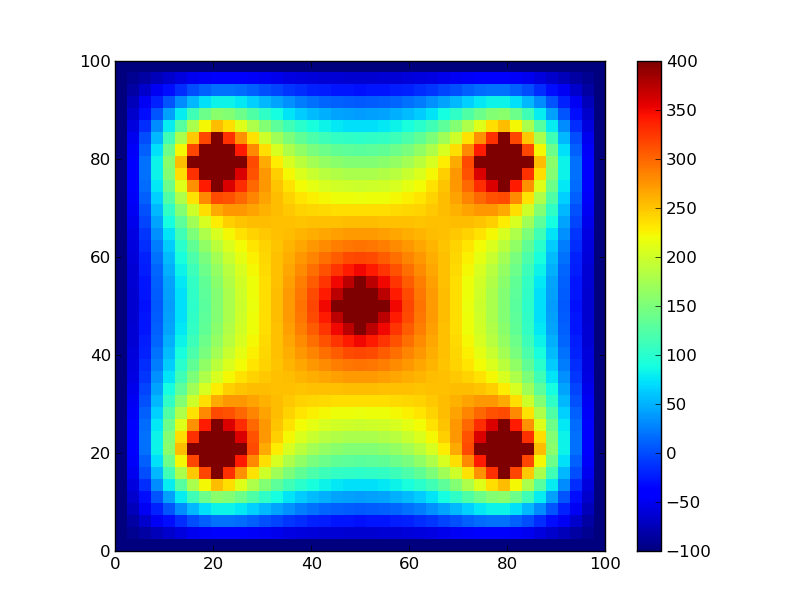
\includegraphics[scale=0.3]{imagenes/test5.png}
                \caption{Granularidad 2.5}
        \end{center}

\end{figure}

Ahora veamos que obtenemos al aplicarle distintas veces el algoritmo de solución random explicado en el desarrollo (\ref{sec:solucionRandom}).

\begin{figure}[htb]

\minipage{0.5\textwidth}
\begin{center}
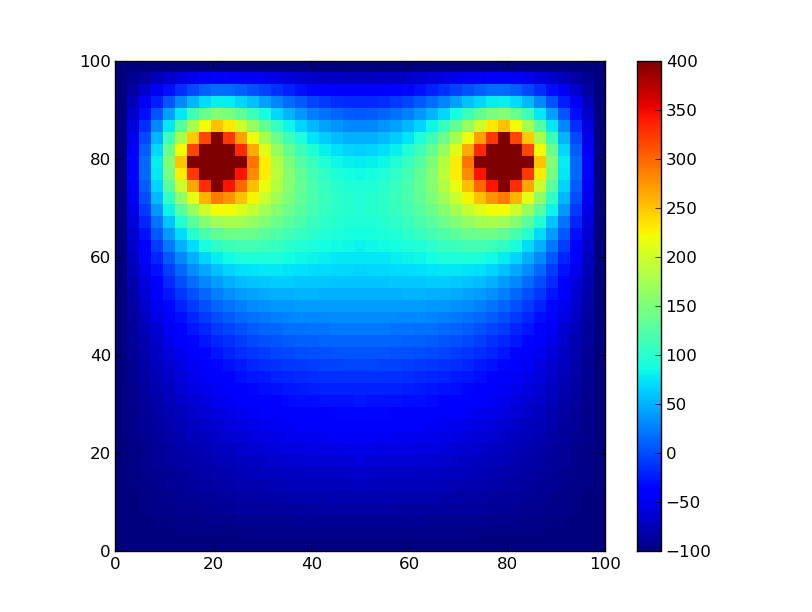
\includegraphics[scale=0.3]{imagenes/random_1.png} 
\caption{Resultado primer corrida} 
        \end{center}
\endminipage\hfill
\minipage{0.5\textwidth}
\begin{center}
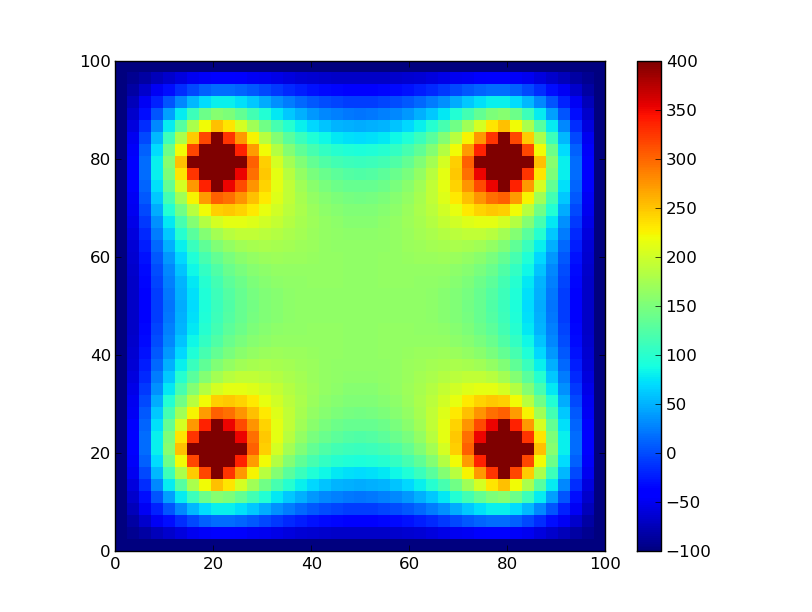
\includegraphics[scale=0.3]{imagenes/random_2.png} 
\caption{Resultado segunda corrida} 
        \end{center}
\endminipage\hfill 
\end{figure}

\begin{figure}[htb]
\begin{center}
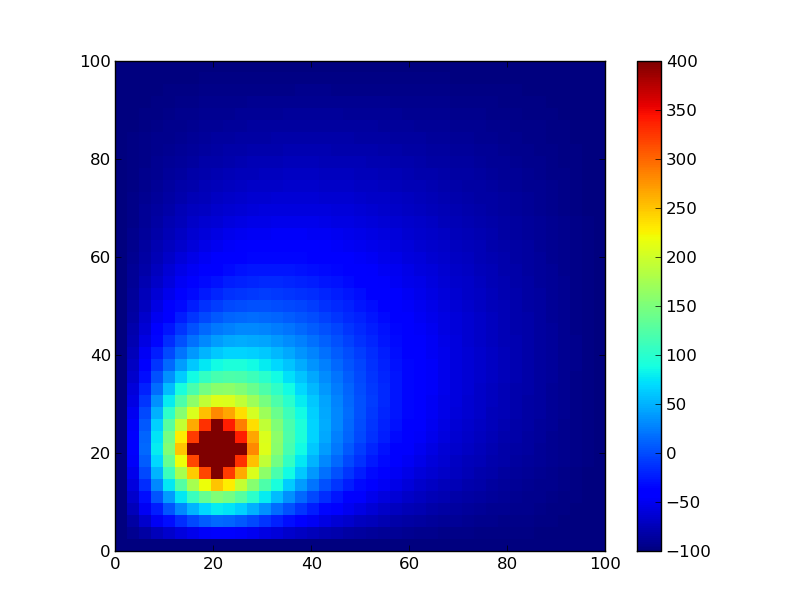
\includegraphics[scale=0.3]{imagenes/random_3.png} 
\caption{Resultado tercer corrida} 
\end{center}
\end{figure}
Como podemos observar la solución óptima (la que menos sanguijuelas elimina), es la segunda. Pero como esta solución es completamente random en la primera corrida mata 2 sanguijuelas antes de elegir 
la correcta y en la tercera 4. Sólo en la segunda elije en el primer intento la sanguijuela correcta. Se aplicó también para todas las granularidades antes mencionadas y se observó el mismo comportamiento erratico a la hora
de matar sanguijuelas. 

\clearpage


\subsubsection{Resultados Greedy}

Veamos ahora para la misma matriz como se comporta nuestro otro algoritmo. 


\begin{figure}[htb]
\begin{center}
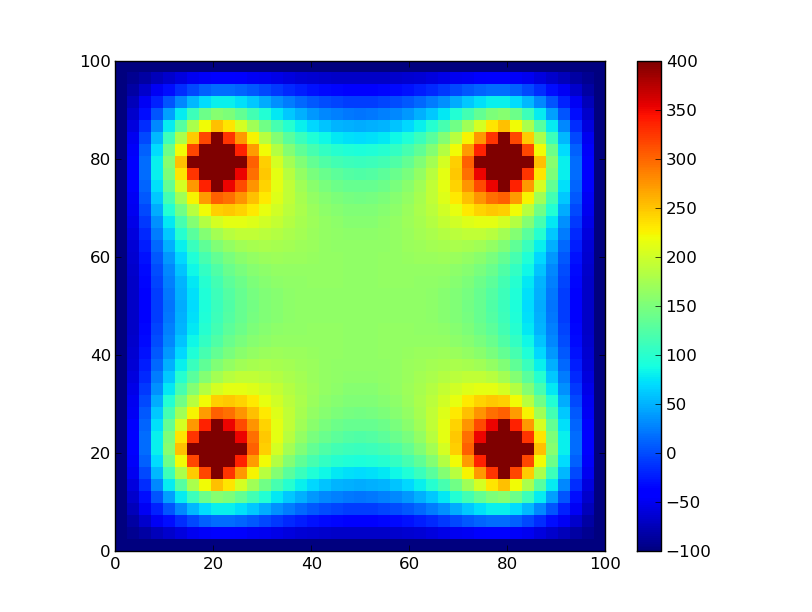
\includegraphics[scale=0.40]{imagenes/random_2.png} 
\caption{Resultado corrida con greedy} 
\end{center}
\end{figure}


En todas las corridas obtuvimos el mismo resultado y demoraron lo mismo. Era de esperarse, ya que efectivamente en este caso, la sanguijuela a eliminar era la del medio.
\newpage
\subsection{Resultados Banda VS Gaussiano}
Veamos ahora que realmente valió la pena la mejora al saber que era matriz banda en cuanto a tiempos en comparación con la eliminación gaussiana.
Anotamos que agregar un análisis de resultados no vale la pena ya que son el mismo

\begin{figure}[htb]
\begin{center}
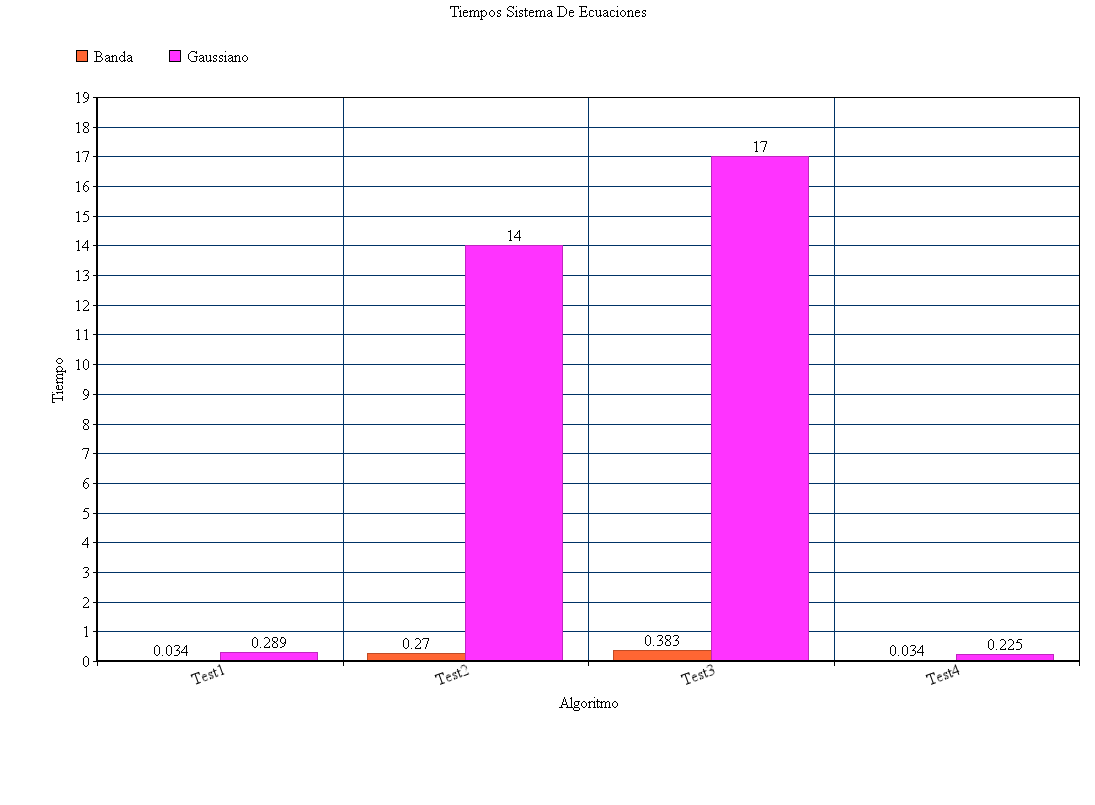
\includegraphics[scale=0.50]{imagenes/tiemposGaussVsBanda.png} 
\caption{Gauss VS Banda} 
\end{center}
\end{figure}
\clearpage
\subsection{Caso solución no es el mas cercano}

A continuación analizaremos un caso en el cual se debe eliminar una sanguijuela que no es la más cercana para efectivamente poder reducir la temperatura en punto crítico.
\begin{figure}[htb]
\begin{center}
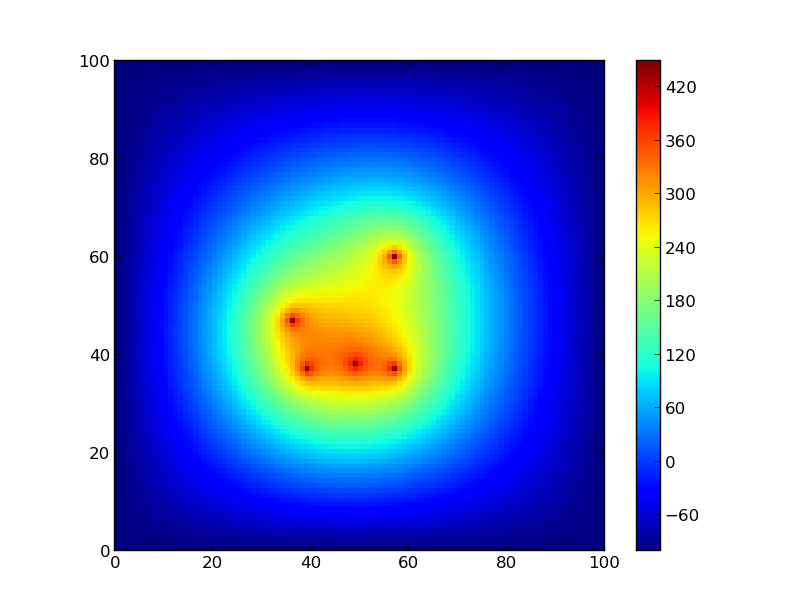
\includegraphics[scale=0.40]{imagenes/test6.png} 
\caption{Parabrisas granularidad 1} 
\end{center}
\end{figure}

Como podemos observar en las imágenes que estan debajo, la solución greedy no es la óptima ya que mató a una sanguijuela extra. Esto es debido a que la principal radiación de calor era producida por el conjunto de 
sanguijuelas que están debajo del punto crítico y no por la mas cercana. Si eliminamos la sanguijuela central de aquel conjunto la radiación de calor emitida por él disminuye drásticamente en el punto crítico produciendo 
que la temperatura esté por debajo de los 235 grados sin necesidad de eliminar a las mas cercana. 

\begin{figure}[htb]
\minipage{0.5\textwidth}
\begin{center}
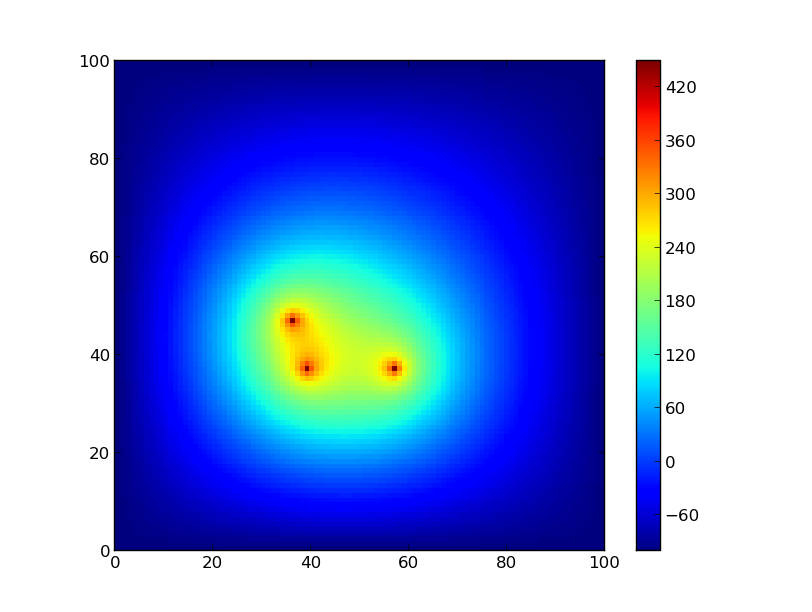
\includegraphics[scale=0.40]{imagenes/test6_greedy.png} 
\caption{Solución Greedy} 

        \end{center}
\endminipage\hfill
\minipage{0.5\textwidth}
\begin{center}
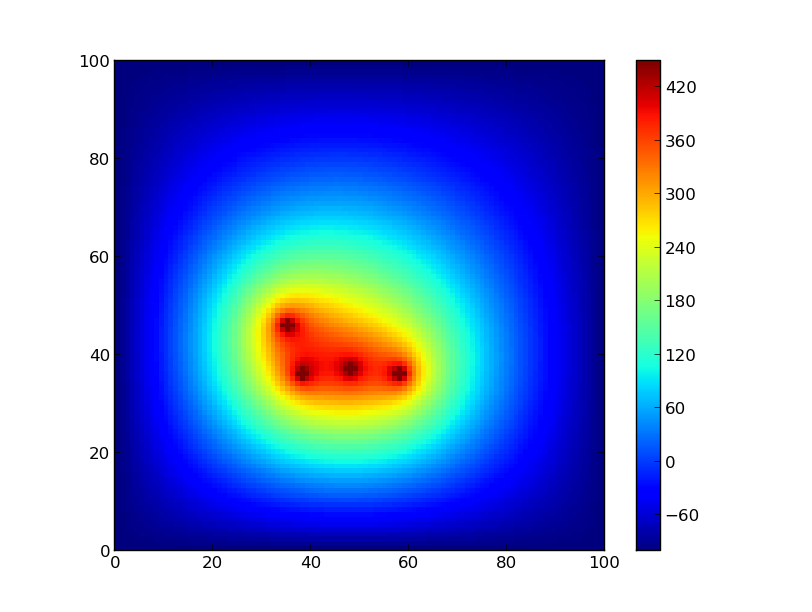
\includegraphics[scale=0.40]{imagenes/test6_solucion_real.png} 
\caption{Solución real} 
        \end{center}
\endminipage\hfill 


\end{figure}
Los datos exactos de este test son:

Medidas: 100 x 100 
discretización:1 
radio: 1.40 
tempreratura sanguijuelas:450 
Posiciónes sanguijuelas:
48 37
58 61
58 36
38 36
35 46



